% % !TEX root =/Users/martabellesmunoz/Dropbox/Documents/Berkley-Standards/Structure.tex

\documentclass[11pt]{article}
\usepackage[colorlinks=true,
			urlcolor=black,
			linkcolor=black,
			citecolor=black
			]{hyperref} 

\usepackage[english]{babel}
\usepackage[utf8]{inputenc}
\usepackage{amsmath, amsthm, amssymb}
\usepackage{enumerate, enumitem}
\usepackage{graphicx}
\usepackage{color, xcolor}
\usepackage{setspace}
\usepackage{hyperref}
\usepackage{authblk}
\usepackage{tikz}
\usetikzlibrary{arrows}
\usetikzlibrary{positioning}
\usepackage{mathtools}
%floor vs. ceil
\DeclarePairedDelimiter{\floor}{\lfloor}{\rfloor} 
\DeclarePairedDelimiter{\ceil}{\lceil}{\rceil}  % If called \ceil*{x} it will add left/right.

%\usepackage{algorithmicx}
\usepackage{algorithm}
\usepackage[noend]{algpseudocode}
\makeatletter
\def\BState{\State\hskip-\ALG@thistlm}
\makeatother
%\usepackage{listings}
%\lstdefinelanguage{Sage}[]{Python}
%{morekeywords={False,sage,True},sensitive=true}
%\lstset{
%  frame=none,
%  showtabs=False,
%  showspaces=False,
%  showstringspaces=False,
%  commentstyle={\ttfamily\color{dgreencolor}},
%  keywordstyle={\ttfamily\color{dbluecolor}\bfseries},
%  stringstyle={\ttfamily\color{dgraycolor}\bfseries},
%  language=Sage,
%  basicstyle={\fontsize{10pt}{10pt}\ttfamily},
%  aboveskip=0.3em,
%  belowskip=0.1em,
%  numbers=left,
%  numberstyle=\footnotesize
%}


\textwidth 16 cm
\textheight 22 cm
\topmargin -1 cm
\oddsidemargin -0 cm

\addtolength{\skip\footins}{1pc plus 5pt} % Foot note space
\setlength\parindent{0pt} % No indent

\newcommand{\N}{\ensuremath{\mathbb{N}}}
\newcommand{\Np}{\ensuremath{\mathbb{N}^{+}}}
\newcommand{\Z}{\ensuremath{\mathbb{Z}}}
\newcommand{\Q}{\ensuremath{\mathbb{Q}}}
\newcommand{\R}{\ensuremath{\mathbb{R}}}
\newcommand{\C}{\ensuremath{\mathbb{C}}}
\newcommand{\Fp}{\ensuremath{\mathbb{F}_p}}
\newcommand{\Fr}{\ensuremath{\mathbb{F}_r}}
\newcommand{\G}{\ensuremath{\mathbb{G}}}
\newcommand{\point}[1]{P_{#1} = (x_{#1}, y_{#1})}
\newcommand{\llog}{\log_2}
\newcommand{\xor}{\oplus}
\newcommand{\minSize}{1.5em}
\newcommand{\gen}[1]{\ensuremath{\langle #1\rangle}}
\newcommand{\noi}{\noindent}

\tikzset{%
	leaf/.style = {draw, fill}, %, minimum size=\minSize},
	empty/.style = {draw},
	wrong/.style = {draw, fill = red},
	internal/.style = {draw, path picture={\draw 
			(path picture bounding box.south east) -- (path picture bounding box.north west) 		(path picture bounding box.south west) -- (path picture bounding box.north east);}}
}

\title{ Sparse Merkle Trees \vspace{-0.2cm} }
\author[1]{Author 1}
\author[2]{Author 2}
\author[1]{Author 3}
\affil[1]{Affiliation 1}
\affil[2]{Affiliation 2}
\date{} %% if you don't need date to appear
\setcounter{Maxaffil}{0}
\renewcommand\Affilfont{\itshape\small}
% 
\includegraphics[scale=0.3]{iden3.png} 

\begin{document}

\maketitle 
\vspace{1cm}
\tableofcontents

\vspace{0.5cm}

%\newpage

\section{Scope}						%% Scope: a section specifying the scope of the standard, highlighting what is being standardized and what is not.
The 4-bit window Pedersen hash function is a secure hash function
which maps a sequence of bits to a point on an elliptic curve \cite{pedersen-gen}.

This proposal aims to standardise this hash function
for use primarily within the arithmetic circuits of zero knowledge proofs,
together with other generic uses such as for Merkle tree or any use cases requiring a secure hash function.

As part of the standard, the paper details the elliptic curve used for the hash function,
the process to compute the Pedersen hash from a given sequence of bits,
and the computation of the hash from a sequences of bits using an arithmetic circuit
---which can be used within zero knowledge proofs.

Moreover the paper contains references to open-source implementations of the 4-bit window Pedersen hash function
which follows the computation process details in this proposal.

%	A section specifying the scope of the standard, highlighting what is being standardized and what is not.
\red{What is the scope here?}

	
\section{Motivation}				%%	A section describing at least one concrete application motivating the proposed standard, including an explanation of why the community will benefit from such a standard.

% FALTEN REFS

The search for an elliptic curve defined over the large prime subgroup of BN128 elliptic curve is motivated by its usefulness in zk-SNARK proofs. We wanted to find a in a deterministic way, so that it was clear no other considerations were taken for defining it. 
With this purpose, we used a deterministic algorithm for finding elliptic curves over a specified finite field together with the restrictions of security parameters of SafeCurves requirements. % requirements s%atisfiability of SafeCurves project. Baby-jubjub is the result of this combination. Baby Jubjub is the result of this research. 
%
%For that, we used a deterministic algorithm done by a group of IRPF researchers in 2016 and EXPOSED IN PAGE SUCH OF \cite{generation-baby}. Baby-jubjub is the result of applying such algorithm.
%
%
%The BN-128 elliptic curve is the curve used in 
%
%Motivation: BN128 elliptic curve has group order SUCH. SNARKs - we look for an elliptic curve defined over the large subgroup of this curve (inside the SNARK, embed, inputs from this group). How to find such a curve, we wanted to do it deterministically, 
%	A section describing at least one concrete application motivating the proposed standard, including an explanation of why the community will benefit from such a standard.

Merkle trees or hash trees are %rooted trees % acyclic connected graphs 
rooted graphs that allow large data be linked by a unique hash value, the hash of the root. Moreover,  a unique set of keys produce a deterministic root hash, regardless of the order in which keys have
been inserted or removed (this is called history independence) [REF].\\

Merkle trees basically en el que cada nodo que no es una hoja está etiquetado con el hash de la concatenación de las etiquetas o valores (para nodos hoja) de sus nodos hijo.
that allow the parent node is the hash of its children, and the leaf nodes are hashes of the original data blocks. A hash tree or Merkle tree is a tree in which every leaf node is labelled with the hash of a data block and every non-leaf node is labelled with the cryptographic hash of the labels of its child nodes [REF]. % A {\bf hash tree} or a {\bf Merkle tree} is an authenticated data structure where every leaf node of the tree contains the cryptographic hash of a data block and every non leaf node contains the concatenated hashes of its child nodes. 
If the *majority* [MORE FORMAL?] of the leaves are empty, then we talk about {\bf sparse Merkle trees}. We actually deal with Sparse Merkle Trees, but we will refer to them simply as Merkle Trees [REF].\\

This way, only a little piece of data is stored on-chain. And with only this piece of data we can check/validate (with negligible error probability) if a certain piece of data is stored in the tree (or not). 
De esta forma proporciona un método de verificación segura y eficiente de los contenidos de grandes estructuras de datos. En sus aplicaciones prácticas normalmente el hash del nodo raíz va firmado para asegurar su integridad y que la verificación sea totalmente fiable. La demostración de que un nodo hoja es parte de un árbol hash dado requiere una cantidad de datos proporcional al logaritmo del número de nodos del árbol.
Hash trees can be used to verify any kind of data stored, handled and transferred in and between computers. They can help ensure that data blocks received from other peers in a peer-to-peer network are received undamaged and unaltered, and even to check that the other peers do not lie and send fake blocks [REF]. proving something is or not in the tree. Merkle trees stuff.
%@book{wikipediansdata,
%title={Data Structures},
%author={Wikipedians, B.},
%url={https://books.google.es/books?id=aYxSZurAGXEC},
%publisher={PediaPress}
%}



% We store (key, values) from people in what so called Merkle trees. This allows us to ... .
%
%The following pages / This document contains the specifications of the Merkle trees implementation used in iden3 and how to generate and verify the proofs. We also add a section explaining per sobre les possibles concerns i blabla. \\

	
\section{Background}				% Background: a section introducing the problem, including definitions, references to previous work and other background details.

The Pedersen hash has already been defined and used by the ZCash team in Sapling,
their latest network upgrade \cite{sapling}.
They construct it on the Jubjub elliptic curve and using 3-bit lookup tables.
In this document, we propose a different implementation of the Pedersen hash function
using Baby-Jubjub elliptic curve and 4-bit windows, which requires less constraints per bit than using 3-bit windows.

%	A section introducing the problem, including definitions, references to previous work and other background details.

Problem: storage of big data structures. Store as minimum information as possible. Reference to previous work and other background details? \\

Definition of (sparse) {\bf Merkle tree}: each node consists of a pair (key, value). Our Merkle trees are binary trees % i.e. at most 2 leaves.
whose nodes consist of pairs {\bf key-value} $(k,v)$. Explain what is a pair key-value. We use them to store claims, which are kept in the leafs and the rest of the nodes furthering up are the hashes of their children. 
Trees have at most 140 levels, that is, a maximum of $2^140$ claims can be stored in them. This number is determined by the length of the hash function used, we will explain later why).\\

% IMPORTANT, MIRAR:
% http://www.diva-portal.org/smash/get/diva2:936353/FULLTEXT02.pdf
% https://eprint.iacr.org/2018/955.pdf
% https://eprint.iacr.org/2016/683.pdf

	
\section{Terminology}				% %	For consistency across documents, adopt throughout the proposal, terminology and definitions used in the ZKProof proceedings, with pointers to the relevant sections.

%	For consistency across documents, adopt throughout the proposal, terminology and definitions used in the ZKProof proceedings, with pointers to the relevant sections.

As we said, (sparse) Merkle trees are such and such:
% Merkle tree
\begin{itemize}
	\item {\bf Merkle tree}
	\item A {\bf Merkle audit path} for a leaf in a Merkle tree is the shortest list of additional nodes in the tree required to compute the root hash for that tree.\\
	
	If the root computed from the audit path matches the true root, then the audit path is a {\bf proof of membership} for that leaf in the tree. [SAY THAT ALSO THE NONCE AND SO ON].
	\item Sparse Merkle Tree (+ pair key-value)
\end{itemize}

Pairs key-value.
\begin{itemize}
	\item Key, value
\end{itemize}

In the tree we distinguish three different nodes (vertices):
\begin{itemize}
	\item {\bf Empty node}: A vertex that stores the value zero.
	\item {\bf Leaf}: A vertex with both empty children. Claims are stored in this kind of nodes. 
	It contains the claim {\color{blue}{i com guarda el key-value (la info que es vol guardar), amb el 1 aquell}}.
	\item {\bf Internal node}: A vertex with at least one non-empty child. It has the hash of its children. If it has one empty child, it keeps the hash of the non-empty one. %Què guarda: els hashos dels seus fills. Si el fill és empty, només es guarda el hash del no buit. 
% and then the nodes further up in the tree 
% Every time a new claim is added to the tree, it is kept in one leaf of the tree and the rest of the nodes 
% furthering up contain the hashes of their children. 
%composed of vertices of $key-value$
% that store the data in their leafs and Nodes further up in the tree are the hashes of their respective children. % All the nodes consist of a pair key-value. 
\end{itemize}

Proofs (definition of a proof The siblings stuff!!):

\begin{figure}[h]
	\centering
	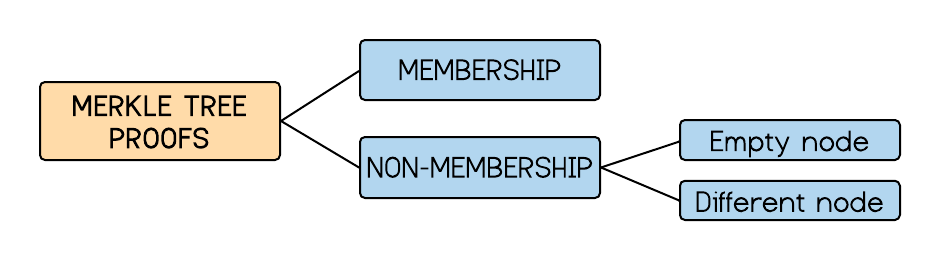
\includegraphics[scale=0.8]{images/MT-pfs-h.png} 
	%	  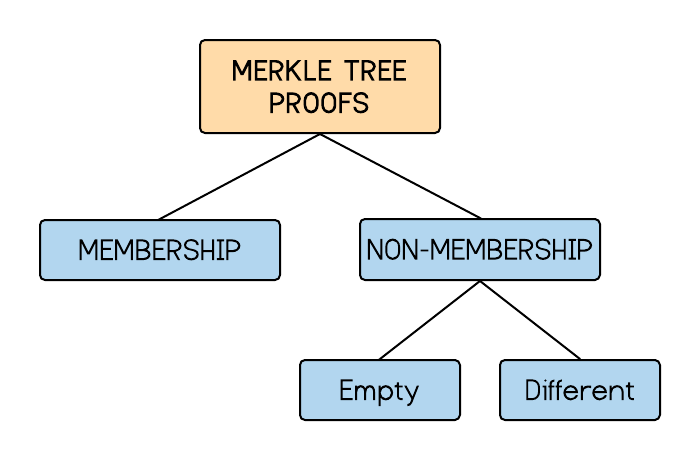
\includegraphics[scale=0.8]{MT-pfs.png} 
	% https://www.lucidchart.com/documents/!
\end{figure}

\begin{itemize}
	\item Proof of membership
	\item Proof of non-membership
	\begin{itemize}
		\item Case 1: empty node
		\item Case 2: different node
	\end{itemize}
\end{itemize}

%\subsubsection{Proof of membership}% !TEX root =/Users/martabellesmunoz/Dropbox/Documents/Especificacions/Merkle trees/Description.tex

Dibuixet + explicacions\\

\begin{center}
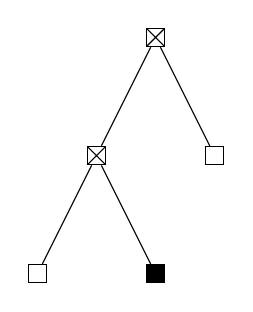
\begin{tikzpicture}[auto,node distance=1.5cm]	 
\node [internal] (r){ }
  child { node [internal]  (a) { }
    		child {node [empty] (c) { }}
    		child {node [leaf] (d) { }}
  	}
  child { node [empty] (b) { } };
\end{tikzpicture}
\end{center}

%\subsubsection{Proof of non-membership}%\subsection{Empty node} 	
% !TEX root =/Users/martabellesmunoz/Dropbox/Documents/Especificacions/Merkle trees/Description.tex

Dibuixet + explicacions\\

\begin{center}
\begin{tikzpicture}[auto,node distance=1.5cm]
	\tikzstyle{internal}  = [draw, path picture={\draw (path picture bounding box.south east) -- (path picture bounding box.north west) (path picture bounding box.south west) -- (path picture bounding box.north east);}]
	\tikzstyle{leaf} = [draw, fill]
	\tikzstyle{empty} = [draw, ]
	\tikzstyle{wrong} = [draw, fill = red]
	 
\node [internal] (r){ }
  child { node [internal]  (a) { }
    		child {node [empty] (c) { }}
    		child {node [empty] (d) { }}
  	}
  child { node [empty] (b) { } };
\end{tikzpicture}
\end{center}

%\subsection{Different node} 	
% !TEX root =/Users/martabellesmunoz/Dropbox/Documents/Especificacions/Merkle trees/Description.tex


Dibuixet + explicacions\\

\begin{center}
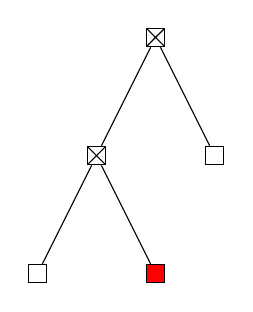
\begin{tikzpicture}[auto,node distance=1.5cm]
	\tikzstyle{internal}  = [draw, path picture={\draw (path picture bounding box.south east) -- (path picture bounding box.north west) (path picture bounding box.south west) -- (path picture bounding box.north east);}]
	\tikzstyle{leaf} = [draw, fill]
	 \tikzstyle{empty} = [draw]
	 \tikzstyle{wrong} = [draw, fill = red]
	 
\node [internal] (r){ }
  child { node [internal]  (a) { }
    		child {node [empty] (c) { }}
    		child {node [wrong] (d) { }}
  	}
  child { node [empty] (b) { } };
\end{tikzpicture}
\end{center}



\section{Challenges}				%% Challenges: for motivating the discussions, highlight the main challenges in creating such a standard,
% as well as any open or unresolved questions.
One of the main challenges to create this standard and to see it adopted by the community is
to provide correct, usable, and well-maintained implementations in as many languages as possible.

Some effort is also required to audit and verify code coming from the community
and claiming to implement the 4-bit window Pedersen hash function
to prevent the propagation of potentially insecure implementations.

Finally, the proposal as it stands today includes the padding of the message $M$ to a multiple of four bits.
There are potentials issues with this approach where collisions can happen.

%For example, the sequences of bits \texttt{10000} and \texttt{10000000} will share the same hash
%as the former pre-image is padded to \texttt{10000000} which is identical to the latter pre-image.
%We were unable to confidently solve this issue in time for the submission deadline of the first draft,
%but this oversight will be solve before the final version is submitted.


 
%	For motivating the discussions, highlight the main challenges in creating such a standard, as well as any open or unresolved questions.

Improve such and such.

We included that hash(0,0)=0.

Com que no anem fins avall de tot, p.m.


% This section is not in the supposed structure of the doc.	
\section{Description}				%	The computation of the Pedersen hash has two steps: first, the generation of the base points $P_0, P_1, \dots, P_5$ (we take $k=5$). This only needs to be done only once, as they can be reused to compute hashes of other data {[REF?]}. Secondly, the calculation of expression (\ref{eq-ped}). We describe in terms of circuits how to do such computation and provide an example explaining both steps.  
	% We describe in terms of circuits and with an example, how to do it. 
	% The circuits used to compute this sum are quite similar to the ones used to calculate the multiple of a point of an elliptic curve except that here we only work with the twisted Edwards form of $E$ and we can have many points precalculated, so instead of doubling all the time, we work with look-up tables. 
	


\subsection{Procedures}
\subsubsection{Storage (INSERTION) (INSERT) of entries}% in the tree}
% Storage of a claim

Let $e$ be a new entry in a tree. The node in which this piece of data is stored is uniquely determined from the data itself. The entries, claims, are arrays of four elements\footnote{{\color{blue}4 field elements of $\mathbb{F}_r$ [{\color{blue}where aquest $r$ és tal}]}}, say $e = e_0, e_1, e_2, e_3$. % consist of four values consists (is of the form) of an array of 
Then we define 
\begin{itemize}
	\item $H_{path} = H(e_2, e_3)$
	\item $H_{value} = H(e_0, e_1)$
\end{itemize}
The first value is a set of bits that is going to represent a path through the tree: starting by the less significant bit and from the root, when we go down one level, we go to the left if there is a 0 and to the right if there is a 1. {\color{blue}TODO: Posar un dibuixet d'exemple.}\\
% to the  0 goes one level down from the left and a 1 takes the right path. 
%bit takes the left child and a 1, the right one. 

Most probably\footnote{\color{blue}es basa en la probabilitat de col·lisió del hash, que és negligible, i posar referència.} we will not go down to the 140th level of the tree, that is, 
%When we want to store a claim : we take $H_{path}$. We will not go down to the 140th level, unless it is necessary. That is, 
we will not use the whole hash, only the necessary amount of bits. What we do is go down through the path until we find a node without siblings (a leaf). If the leaf is empty, we store $e$. Otherwise, that vertex stores some other claim $e'$ (as non-empty leafs store claims). This means that $H_{path}$ and $H'_{path}$ start with the same sequence of bits. What we do is that we 
% go down the tree with both claims until the first different bit and 
compare these two values and find the first different bit (included). Then we store the claims in the leafs resulting of the path up to that bit (included). 
%
This process of storing an entry $e$ in a tree $T$ with root $r$ is explained in the following pseudocode (code?).\\
%, this is the way to store a new entry $e$ in a tree $T$ with root $r$.\\
% We continue 
% and the first node without siblings, is our position. If there is a coincidence, osigui, si on hem d'anar hi ha algun node, hem de mirar la seva $H_pos$ i esplitar fins el primer número que no coincideixi. 
%until we find a node without siblings. There, we store 

%In order of lsb: $k_i = 0$ -> left, and 1 -> right. An *EXAMPLE* of a hash that would determine the position. Actually, only the necessary amount of bits! :) 

%So, in our tree there will be three types of vertices: 
% Explicar com va: hi ha tres tipus de nodes --> Buit, etc.

%In our case, these data will be claim that will consist in an array of 4 ... : $[e0, e1, e2, e3]$ and we will do $this and that for$ $H_pos$ i tal. So, Hpos is a set of bits that will represent a path through the tree.\\

% The information will be stored in leaves of the tree. \\

%, except for the leaves (although implicitly, they do). 
% A hash tree is a tree of hashes in which the leaves are hashes of data blocks in, for instance, a file or set of files.  For example, in the picture hash 0 is the result of hashing the concatenation of hash 0-0 and hash 0-1. That is, hash 0 = hash( hash 0-0 || hash 0-1 ) where || denotes concatenation. 


% \subsection{Leafs (storage of stuff)} %(claims or roots, which are also claims...))

%Each leaf of the tree stores the pair (key, value)=$(k, v)$ where $k = H_{tot}$. And the extra 1 thing, as it is *terminal* (neh?) node. 

% \subsection{Internal nodes}

%El hash és $H([\#, k_i, v_i])$, on $\# = 1$ if terminal node (leaf) and $\# = 0$ if not.

%\begin{itemize}
%	\item Hash of (left, right) -> concatenated? Mirar el Hash i tal.
%\end{itemize}



% 
% The first value $H_{pos}$ converted to binary (spec) determinates the position in which the value is stored. The second hash $H_{tot}$ is the key associated to $v$ that will be stored together with $v$.

%$$ ESCRIURE-AQUi-UN-LOOP. $$
% Arbre, l'entrada és un key value $(k,v)\in F^2$. ( p is a prime of 256 bits)

% En GoLang (Edu):
% https://github.com/iden3/go-iden3/blob/master/merkletree/merkletree.go#L260
\begin{algorithm}
	\begin{algorithmic}[1]
		\setstretch{1.2}
		\Procedure{Insert Entry $e$ in Merkle Tree $T$ with Root $r$}{}
		%
		\State $H_{path} \gets \text{GetPath($e$)}$
		\State $b \gets \text{LeastSignificantBit($H_{Index}$)}$
		%
		\If {$r$ is empty} $r \gets e$
		\Else
		\While{$r$ is internal vertex} 
		\If {$b=0$} {$r \gets \text{LeftChild($r$)}$}
		%		\EndIf
		\Else { $r \gets \text{RightChild($r$)}$} %\If{$b=1$} (alternatively)
		\EndIf
		\If {$r$ is empty}
		\State $r \gets e$
		\State $H_{Index} \gets H_{Index}\backslash{b}$
		\State $b \gets \text{LeastSignificantBit($H_{Index}$)}$
		\EndIf	
		\EndWhile
		\EndIf
		%
		\State $e' \gets \text{GetEntryStoredIn($r$)}$
		\State $H'_{path} \gets \text{GetPath($e'$)}$
		\If {$H_{path} \not= H'_{path}$}
		\State Find first bit $b_j$ such that $H_{path}(j) \not= H'_{path}(j)$
		\State Leaf($b_0...b_j$)$\gets e$ %Store $e$ in Position$(b_0...b_j)$
		\State Leaf($b_0...b'_j$)$\gets e'$ %Store $e'$ in Position$(b_0...b'_j)$
		\State RecalculateIntermediateNodeValues($T$)	
		\EndIf
		\EndProcedure
	\end{algorithmic}
\end{algorithm}

Once it is saved, then we take then we construct the leaves up the following way: el tema dels hashos, que es concatena tal i que si hi ha un zero, doncs que llavors només el hash del fill no buit. Then, the rest of intermediate nodes need to be recalculated (as they are hashes of changed children). \\

Note depth is not fixed (at the beginning, it keeps changing). Limit de l'arbre -> tants nivells com números retorna el hash (with is MiMC7, for now). \\
%The position of the (k,v) is determined by ... .
%\begin{enumerate}
%	\item First storage: we "create" a root
%	\item Then: ...
%	\item If (k,v) and k1,v1 , k2 and k1 coincide (collision resistant), but some values do so: lsb thing... .
%\end{enumerate}

% Note that the height of the tree is not fixed from the beginning. It varies when we add stuff. Nevertheless, as MiMC returns a 256-bit string, the trees are bounded to 256 levels. (REMARK that a collision of 256 has negligible probability).
% A partir de quan hi ha col·lisions?


% For a proof, give the necessary siblings. If there is no sibling --> we give a 0 back.
+ EXAMPLE.

\subsubsection{DELETE of entries}% in the tree}
+ EXAMPLE.

\subsubsection{UPDATE the tree}% in the tree}
+ EXAMPLE.

\subsection{Verification of proofs}
Given a blabla. 

\section{Security}					%%	If relevant, provide a proof of security in the description.
%	If relevant, provide a proof of security in the description.


Afegir aquí que no pot lie (perquè se li requereix l'altre hash i tal). Examples if one lies.

QUE FALTA CALCULAR LA PROBABILITAT DE COL·LISIÓ.

+ Make sure we go all the tree down to a leaf (that extra 1).

Suppose the queries know the info (the claim).

We do not delete stuff.

The  security  of  an  audit  path  reduces  to  the  collision  resistance  of the underlying hash function $H$.
Proof.: %https://eprint.iacr.org/2016/683.pdf#cite.Mer%3A87%3AA, Lemma1 (page 3, sec.2.2)

\section{Implementation}			%%	If relevant, submit an open source prototype implementation (by including a reference to the repository with the code).

% Others (entry?)
Nonce? of a claim?

Types of entries: claims, etc. D'una part en treiem el lloc on ho guardem i a l'altre etc.
Such implementation in GoLang and in JavaScript. \\

The entries are pairs key-value.\\

Example from iden3 documentation.
%	\subsection{Hash}				
%Our elements are of : 

%	, where 
%	$$ r = 	21888242871839275222246405745257275088548364400416034343698204186575808495617 $$
% The hash function used in the Merkle tree is MiMC-7 described in \cite{mimc}.\\
%[REF]. Original paper MiMC hash: \url{https://eprint.iacr.org/2016/492.pdf}.\\
The hash function used in EdDSA is MiMC-7 based in paper \cite{mimc}, which describes the hash using exponent 3. In this specification, we use exponent 7 (hence the name MiMC-7) as 3 and $l-1$ are not coprime and 7 is the optimal choice for exponentiation \cite[Sec. 6]{mimc}.\\

% and goes as follows: %is constructed as follows: 
%
Let $\Fl$ be the finite field with $l$ elements. The block cipher is constructed by iterating a round function $r$ times where each round consists of a key addition with the key $k$, the addition of a round constant $c_i\in \Fr$, and the application of a non-linear function defined as $F(x) :=x^7$ for $x\in \Fl$. The ciphertext is finally produced by adding the key $k$ again to the output of the last round. Hence, the round function is described as $F_i(x) = F(x) \xor k \xor c_i$ where $c_0 = c_r = 0$ and the encryption process is defined as 
	$$ 
		E_k(x) = (F_{r-1} \circ F_{r-2} \circ ... \circ F_0)(x) \xor k.
	$$


%. Instead the constants are fixed once and can be hard-coded into the implementation on either side. 


%The number of rounds is: 
%$$ \text{nRounds} = \ceil*{\frac{\llog r}{\llog 7}} = 91. $$\\

%% Esquema MIMC-7
% !TEX root =/Users/martabellesmunoz/Dropbox/Documents/Especificacions/Merkle trees/Description.tex

\tikzstyle{exp} = [draw, minimum size=2em] % fill=blue!20,
\tikzstyle{init} = [pin edge={to-,thin,black}]
\tikzset{XOR/.style={draw,circle,append after command={
        [shorten >=\pgflinewidth, shorten <=\pgflinewidth,]
        (\tikzlastnode.north) edge (\tikzlastnode.south)
        (\tikzlastnode.east) edge (\tikzlastnode.west)
        }}
}

\begin{center}
\begin{tikzpicture}[node distance=1.5cm, auto,>=latex']

    \node  (in) {$x$};
    \node [XOR, pin={[init]above:$k$}] (xor0) [right of=in, node distance=1cm]  { };
    \node [exp] (e0) [right of=xor0] {$x^7$};
    \node [XOR, pin={[init]above:$k \oplus c_1 $}] (xor1) [right of=e0] { };
    \node [exp] (e1) [right of=xor1] {$x^7$};
    \node [XOR, pin={[init]above:$k \oplus c_{r-1} $}] (xorr-1) [right of=e1, node distance=4cm] { };
    \node [exp] (er-1) [right of=xorr-1] {$x^7$};
    \node [XOR, pin={[init]above:$k \oplus c_r $}] (xor)  [right of=er-1] { };
    \node  (out)  [right of=xor, node distance=1cm] {$y$};

    \path[->] (in) edge node { } (xor0);
    \path[->] (xor0) edge node { } (e0);
    \path[->] (e0) edge node { } (xor1);
    \path[->] (xor1) edge node { } (e1);
    \path[->] (e1) edge[dotted] node { } (xorr-1);
    \path[->] (xorr-1) edge node {} (er-1);
    \path[->] (er-1) edge node { } (xor);
    \path[->] (xor) edge node { } (out);
   
\end{tikzpicture}
\end{center}


As the random  constants $c_i$ do  not  need  to  be  generated  for  every evaluation of MiMC-7, they are hard-coded into the implementation. The generation of these constants and the required number of rounds is described in section \ref{sec-mimc}. 
%
%The hash returns 140 bits, this is why Merkle trees are bounded by 140 levels (it is the length of the whole path of a claim). \\
%
%Encadenar valors (tipu pel hash de H(v1, v2, v3, v4) etc.\\

%	\subsection{Example}			 







%\begin{center}
%\begin{tikzpicture}[auto,node distance=1.5cm] %, sibling distance=10em]
%%  level distance=20mm,
%%  text depth=.1em,
%%  text height=.8em,
%%  level 1/.style={sibling distance=10em},
%%  level 2/.style={sibling distance=20em},
%%  level 3/.style={sibling distance=20em},
%%  level 4/.style={sibling distance=10em}]
% \node [internal] (a){ } %root
%  child { node [internal]  (b) { }
%    		child {node [internal] (d) { }
%			child {node [leaf] (h) { }}
%			child {node [leaf] (i) { }}
%			}
%    		child {node [empty] (e) {asdfasdf }}
%  	}
%   child { node [internal] (c) { }
%    		child {node [empty] (f) { }}
%    		child {node [internal] (g) { }
%			child {node [internal] (j) { }
%				child{node [leaf, fill = green] (l) { } }
%				child{node [leaf] (m) { } }
%			}
%			child {node [empty] (k) { }}	
%		}
%  	};
%\end{tikzpicture}
%\end{center}

	
	
\section {Intellectual Property}	%	We aim to ensure that proposals can be freely implemented. Thus, proposals should disclose the existence of any known patents (awarded or pending) which may restrict free implementation. This may affect the decision process, and a detailed policy is being developed.

%\newpage
%\addcontentsline{toc}{section}{References}
%\bibliographystyle{acm}
%\bibliography{lit}

\end{document}